% vim: set spell spelllang=es syntax=tex :

\documentclass[11pt,a4paper,spanish]{beamer}

\usepackage[spanish]{babel}

\usepackage[utf8]{inputenc}

\usepackage{graphicx}

\usepackage{subcaption} %Para Subfigure

\usepackage{caption} %Para captions en las figuras sin prefijo

\usepackage{upquote} % Para comillas rectas en verbatim
\usepackage{fancyvrb}

\usepackage{ccicons}

\usepackage{url}

\usepackage{babelbib}

\usefonttheme{serif}

\setlength{\parskip}{1.5mm}

\newcommand{\cw}[1]{\mbox{\texttt{\textcolor{blue}{#1}}}}
\newcommand{\dq}[0]{\Verb+"+}
\newcommand{\sq}[0]{\textquotesingle}

\usetheme{Rochester}
\usecolortheme{whale}

%\usetheme{Warsaw}

\beamertemplatenavigationsymbolsempty

\setbeamertemplate{background canvas}{
    \raisebox{-0.99\paperheight}[0pt][0pt]{
        \makebox[\paperwidth]{
            \null
            \hspace{-1em}
            \includegraphics[width=0.09\paperwidth]{logos/fai.pdf}
            \hspace{0.8\paperwidth}
            %\hfill
            \hspace{-1em}
            \includegraphics[width=0.09\paperwidth]{logos/uncoma.pdf}
            }
    }
}

\title{\textbf{\texttt{Shell UNIX}}}

\author{}

\date{}

\defbeamertemplate{footline}{centered page number}
{
    \hspace*{\fill}
    \usebeamercolor[fg]{blue}
    \usebeamerfont{page number in head/foot}
    \insertpagenumber\,/\,\insertpresentationendpage
    \hspace*{\fill}\vskip2pt
}
\setbeamertemplate{footline}[centered page number]

\begin{document}

\begin{frame}[noframenumbering]

    \maketitle
    \centering
    \vspace{-8em}~
    \begin{figure}
    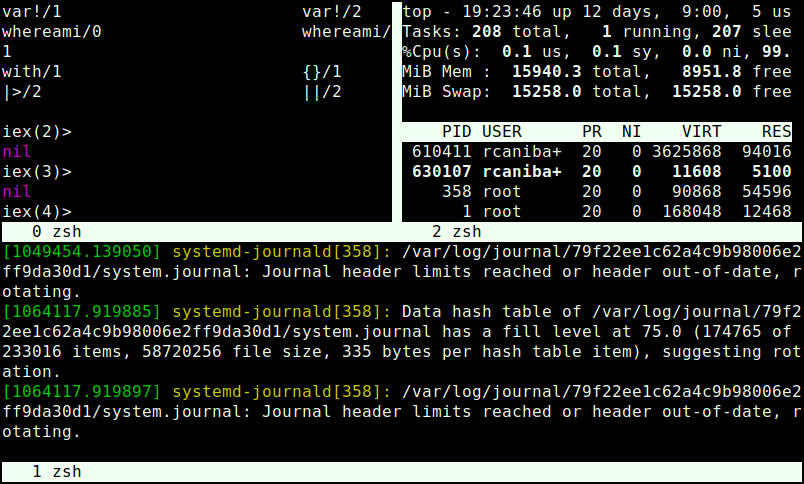
\includegraphics[height=0.55\textheight]{img/screen.pdf}
    \end{figure}

\end{frame}

\begin{frame}[label=temario]

    \frametitle{Temario}

\begin{itemize}

    \item ¿Qué es un \emph{shell}?
    \item Interpretes por linea de comandos.

    \item Sintaxis básica.
        \begin{itemize}
            \item Variables de entorno.
            \item Caracteres especiales:
            \begin{itemize}
                \item Control de de ejecución.
                \item Comillas y barra invertida.
            \end{itemize}
        \item Patrones y comodines.
        \item Redirección:
            \begin{itemize}
                \item A archivos.
                \item El \emph{pipe} \cw{|}.
            \end{itemize}
        \item Substitución de comando.
        \end{itemize}
    \item \cw{grep}

\end{itemize}

\end{frame}

\begin{frame}

    \frametitle{Administración de sistemas}
    \framesubtitle{Definición \emph{shell}}

    El \emph{Shell} de un sistema es un proceso que funciona de interfaz
    entre el usuario y la computadora. Puede ser de solo texto o gráfico.

    \begin{figure}
    \centering
    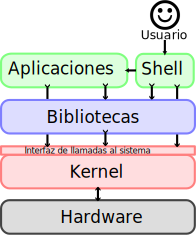
\includegraphics[height=0.65\textheight]{img/os.pdf}
        \captionsetup{textfont=tiny,labelformat=empty,justification=centering}
        \caption{}
    \end{figure}

\end{frame}

\begin{frame}

    \frametitle{Interpretes de linea de comandos}

    Interfases que lee e interpreta lineas de texto.

    \begin{itemize}
        \item \textbf{Shell POSIX}: \cw{sh}, \cw{ash},
            \cw{bash}, \cw{zsh}.
        \item \cw{csh}: estructuras similares a \cw{C}.
        \item \cw{fiSH}: enfocado a interactividad y facilidad de uso.
    \end{itemize}

\end{frame}

\begin{frame}

    \frametitle{Interpretes de linea de comandos POSIX}
    \framesubtitle{Sintaxis básica}

    \begin{figure}
    \centering
    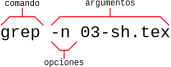
\includegraphics[width=0.80\textwidth]{img/sintaxis.pdf}
    \end{figure}

    \begin{itemize}
        \item Los argumentos están separados por un espacio en blanco.
        \item Múltiples espacios en blanco consecutivos se ignoran.
        \item Si alguno de los argumentos tiene espacios, estos deben ser
            ``escapados''.
    \end{itemize}

\end{frame}

\begin{frame}

    \frametitle{Interpretes de linea de comandos POSIX}
    \framesubtitle{Variables de entorno}

    \begin{itemize}
        \item Nombres asociados a cadenas de texto.\pause
        \item Se definen con el formato \cw{nombreVariable=Valor}, sin
            espacios entre el símbolo igual y el nombre, ni entre el igual y
            el valor.
        \begin{itemize}
            \item[Ejemplo:] \cw{miVariable=Hola}\pause
        \end{itemize}
        \item Se accede al valor de la variable anteponiendo un signo pesos al
            nombre de la variable.
        \begin{itemize}
            \item[Ejemplo:] \cw{echo \$miVariable} imprime
                \cw{Hola}\pause
        \end{itemize}
        \item Existen variable ya pre definidas, como \cw{USER},
            \cw{PWD}, y \cw{TERM}. Se pueden ver todas con el
            comando \cw{set}.\pause
        \item Para poder ser accedidas por procesos hijos, deben ser
            exportadas con el comando \cw{export}.
        \begin{itemize}
            \item[Ejemplo:] \cw{export miVariable}
        \end{itemize}
    \end{itemize}

\end{frame}

\begin{frame}

    \frametitle{Interpretes de linea de comandos POSIX}
    \framesubtitle{Caracteres especiales: control de ejecución}

    \begin{itemize}
        \item Punto y coma (\cw{;}) permite delimitar múltiples comandos
            en una sola linea.
        \begin{itemize}
            \item[Ejemplo:] \cw{date; who; ls}\pause
        \end{itemize}
    \item \textbf{AND} (\cw{\&\&}) el segundo comando solo se ejecutara
        si el primero tiene éxito.
        \begin{itemize}
            \item[Ejemplo:] \cw{true \&\& echo OK} imprimirá \cw{OK}.
            \item[Ejemplo:] \cw{false \&\& echo OK} no imprimirá \cw{OK}.
            \pause
        \end{itemize}
    \item \textbf{OR} (\cw{||}) el segundo comando solo se ejecutara si
        el primero falla.
        \begin{itemize}
            \item[Ejemplo:] \cw{true || echo FAIL} no imprimirá \cw{FAIL}.
            \item[Ejemplo:] \cw{false || echo FAIL} imprimirá \cw{FAIL}.
            \pause
        \end{itemize}
    \item Paréntesis  (\cw{()}) y llaves (\cw{\{\}}) permiten
        agrupar comandos.
        \begin{itemize}
            \item[Ejemplo:] \cw{\{cd /; touch file\} \&\& echo OK}
                imprimirá \cw{OK} solo si el último comando tuvo éxito.
        \end{itemize}
    \end{itemize}

\end{frame}

\begin{frame}

    \frametitle{Interpretes de linea de comandos POSIX}
    \framesubtitle{Caracteres especiales: Comillas y barra invertida}

    \begin{itemize}
        \item Barra invertida (\cw{\textbackslash}) le indica al
            interprete que el caracter siguiente debe ser interpretado como
            texto.
        \begin{itemize}
            \item[Ejemplo:] \cw{echo
                \textbackslash{};\textbackslash{}\$O}
                imprime \cw{;\$O}.
            \item[Ejemplo:] \cw{cat mi\textbackslash{} archivo.txt}
                muestra los contenidos del archivo \cw{mi archivo.txt},
                mientras que \cw{cat mi archivo.txt} muestra los
                contenidos de los archivos \cw{mi} y
                \cw{archivo.txt}.\pause
        \end{itemize}
    \item Comillas simples (\cw{\sq{}}) limitan una cadena literal.
        \begin{itemize}
            \item[Ejemplo:] \cw{echo \sq{}Hola \$Mundo!!;\sq{}}
                imprimirá \cw{Hola \$Mundo!!;}.\pause
        \end{itemize}
    \item Comillas dobles (\cw{\dq{}}) limitan una cadena en la que las
        variables serán remplazadas. Se pueden encerrar el nombre entre llaves
            para separarla del texto circulante.
        \begin{itemize}
            \item[Ejemplo:] \cw{miVar=\dq{}Mundo\dq{}; echo \dq{}Hola
                \$miVar\dq{}} imprimirá \cw{Hola Mundo!!}.
            \item[Ejemplo:] \cw{miVar=\dq{}Mun\dq{}; echo \dq{}Hola
                \$\{miVar\}do\dq{}}
                imprimirá \cw{Hola Mundo!!}.
        \end{itemize}
    \end{itemize}

\end{frame}

\begin{frame}

    \frametitle{Interpretes de linea de comandos}
    \framesubtitle{Patrones y comodines}

    El \cw{Shell} provee herramientas que permiten hacer referencia a
    múltiples archivos y directorios de una manera concisa utilizando
    patrones. El \cw{Shell} remplaza el patrón por el nombre de los
    archivos o directorios del directorio actual que coincidan este antes de
    ejecutar comando.

    \begin{itemize}
        \item[Ejemplo:] Si el directorio actual contiene los archivos
            \cw{file00 file01} y se lanza el comando
            \cw{cat file*}, el \cw{Shell} ejecutara el comando con
            los argumentos \cw{file00} y \cw{file01}. El proceso
            no vera los comodines.
    \end{itemize}

\end{frame}

\begin{frame}

    \frametitle{Interpretes de linea de comandos}
    \framesubtitle{Patrones y comodines}

    \begin{itemize}
        \item Asterisco (\cw{*}) comodín que concuerda con cualquier
            cadena de texto.
        \begin{itemize}
            \item[Ejemplo:] Si el directorio actual contiene los archivos
                \cw{a.jpg b.jpg a.txt}, el patrón \cw{*} sera
                remplazado por \cw{a.jpg b.jpg a.txt}, mientras que el
                patrón \cw{*.jpg} sera remplazado por \cw{a.jpg
                b.jpg }.\pause
        \end{itemize}
        \item Signo pregunta (\cw{?}) comodín que concuerda con
            cualquier caracter.
        \begin{itemize}
            \item[Ejemplo:] Si el directorio actual contiene los archivos
                \cw{aa ab a b}, el patrón \cw{?} sera remplazado
                por \cw{a b}, mientras que el patrón \cw{??} sera
                remplazado por \cw{aa ab}.\pause
        \end{itemize}
        \item Conjuntos (\cw{[abc]} o \cw{[RANGO]}) comodín que concuerda con
            único caracter dentro de un conjunto (o rango) de caracteres.
        \begin{itemize}
            \item[Ejemplo:] Si el directorio actual contiene los archivos
                \cw{a0 a1 ... a9 b0 b1 ... b9 c0 c1 ... c9}, el patrón
                \cw{[ac][2-4]} sera remplazado por \cw{a2 a3 a4 c2
                c3 c4}.
        \end{itemize}
    \end{itemize}

\end{frame}

\begin{frame}

    \frametitle{Interpretes de linea de comandos}
    \framesubtitle{Redirección}

    Ademas de los argumentos y archivos, los procesos tienen tres canales de
    comunicación: la entrada estándar, la salida estándar y la salida de error
    estándar. La primera esta usualmente asignada al teclado, mientras que las
    otras dos tienen por lo general como destino la pantalla.

    Existen operadores que permiten al usuario cambiar la fuente o destino
    utilizando varios operadores.

\end{frame}

\begin{frame}

    \frametitle{Interpretes de linea de comandos}
    \framesubtitle{Redirección: a archivos}

    \begin{itemize}
        \item Redireccionar la entrada estándar (\cw{<}) cambia la
            fuente al archivo especificado.
        \begin{itemize}
            \item[Ejemplo:] Si se ejecuta \cw{wc </etc/fstab}, el
                proceso tomara como entrada estándar el contenido del archivo
                \cw{/etc/fstab}.
        \end{itemize}\pause
        \item Redireccionar la salida sobreescribiendo el archivo, con
            \cw{>} o \cw{1>} para la salida estándar, y
            \cw{2>} para la salida estándar de error.
        \begin{itemize}
            \item[Ejemplo:] Si se ejecuta \cw{ps > miArchivo}, el
                proceso creara un nuevo archivo llamado \cw{miArchivo}
                donde se volcaran lo que normalmente se mostraría por
                pantalla.
        \end{itemize}\pause
        \item Redireccionar la salida concatenando al archivo, con
            \cw{>>} o \cw{1>>} para la salida estándar, y
            \cw{2>>} para la salida estándar de error.
        \begin{itemize}
            \item[Ejemplo:] Si se ejecuta \cw{ps >> miArchivo}, el
                proceso volcaran lo que normalmente se mostraría por
                pantalla al final del archivo \cw{miArchivo}.
        \end{itemize}
    \end{itemize}

\end{frame}

\begin{frame}

    \frametitle{Interpretes de linea de comandos}
    \framesubtitle{Redirección: el \emph{pipe}}

    Las tuberías o \emph{pipes} (\cw{|}) permiten redirigir la salida
    estándar de un proceso a la entrada estándar del siguiente.

    \begin{itemize}
        \item[Ejemplo:] Si se ejecuta \cw{ps | wc} la salida del proceso
            \cw{ps} sera tomada como entrada del proceso \cw{wc}.
    \end{itemize}

\end{frame}

\begin{frame}

    \frametitle{Interpretes de linea de comandos}
    \framesubtitle{Substitución de comandos}

    La sustitución de comando permite tomar la salida de un proceso como
    argumento para otro. Existen dos variantes: la que delimita el proceso a
    substituir con comillas invertidas (\cw{\`{}}) y la que lo delimita
    el inicio de las sustitución con \cw{\$(} y el final con
    \cw{)}. La segunda versión es la recomendada, ya que permite
    anidar substituciones, y tienen limites más claros.

    \begin{itemize}
        \item[Ejemplo:] Si la salida del comando \cw{whoami} es
            \cw{peperina}, ejecutar \cw{echo \dq{}Hola
            \$(whoami)\dq{}} imprimirá \cw{Hola Peperina}.
    \end{itemize}

\end{frame}

\begin{frame}

    \frametitle{Interpretes de linea de comandos}
    \framesubtitle{\emph{grep}}

    \cw{grep} es una herramienta que permite buscar patrones de
    expresiones regulares en textos (tanto archivos como flujos de texto).
    Las expresiones regulares que soporta son mucho más avanzadas que los
    patrones que soporta el \cw{Shell}\footnote{Consulte el manual:
    \cw{man grep}}, pero para comenzar utilizaremos aquellas
    compatibles.

    \begin{itemize}
        \item[Ejemplo:] Para poder encontrar todas las lineas que contengan
            las palabras \emph{alumno}, \emph{alumna} y \emph{alumne} en los
            archivos \cw{arch1} y \cw{arch2}, podemos ejecutar
            \cw{grep -e alumn[aeo] arch1 arch2}.
        \item[Ejemplo:] Para poder encontrar todos los procesos del usuario
            \emph{peperina} podemos ejecutar \cw{ps aux | grep peperina}.
    \end{itemize}

\end{frame}

\againframe{temario}

\begin{frame}

\title{¿Consultas?}
\maketitle

\end{frame}
%
%\newcounter{lastPage}
%\setcounter{lastPage}{\number\value{page}}
%
%\begin{frame}%[allowframebreaks]
%
%\frametitle{Atribuciones}
%
%\bibliographystyle{abbrv}
%\setbeamertemplate{bibliography item}{\insertbiblabel}
%\tiny
%\bibliography{refimg}
%\end{frame}
%
%\setcounter{page}{\number\value{lastPage}}

\end{document}
